%!TEX root = ../main.tex

\chapter{The ns-3 network simulator}
\label{chp:ns3}

\paragraph{}
The study behind this work required a thorough evaluation of a multitude of different non-terrestrial communication scenarios, that in turn required an extensive simulation campaign. Furthermore, the low-level nature of the issues that were expected to be found led to the need for a simulator that allowed access to the protocols' core implementation to be able to modify their behavior if needed. A simple API-level access to some protocols' attributes would have been not sufficient to implement the suggested modifications.

\section{Description}
\label{sec:ns3_desc}

\begin{figure}[ht]
    \centering
    
\includegraphics[width=0.5\textwidth]{res/ns-3-notext.png}
    \caption{ns-3 logo \href{https://www.nsnam.org/}{nsnam.org}}
    \label{fig:ns3-logo}
\end{figure}

Being a modular, extensible, community-supported, full-stack network software simulation tool based on a discrete event approach, the ns-3 simulator was the software of choice to conduct the testing campaigns. It is an open source project, licensed under the GNU GPLv2 license, meaning that the condition of being able to have full access to the source code to implement potential modifications is satisfied \cite{ns3-website}.

Other simulation pieces of software are available, such as OMNET++ (\href{https://omnetpp.org/}{omnetpp.org}), SWANS (\href{http://jist.ece.cornell.edu/}{jist.ece.cornell.edu}), NetSim (\href{https://www.tetcos.com/}{tetcos.com}), QualNet, and finally ns-3 predecessor, ns-2. Their main characteristics are summarized in Table \ref{tab:simulators}, from \cite{review-ns3}, which highlighted the suitability of ns-3 for research purposes, highlighting its success amongst the scientific community.

\subsubsection{Discrete events simulators}
In discrete-events simulators, each operation to be performed is associated to an event, and in turn, each event is associated with a set of instructions and its execution time. 

The simulation proceeds by processing and executing events, stepping from one to the next, as the simulation time passes. At the eyes of the simulation, each event is executed in zero time, since the time is stopped while executing a single event, and its course resumes only when transitioning between events scheduled at different times.

If no events are scheduled to execute for a certain period of time, the simulation immediately transitions to the next scheduled one. This behavior is the main difference with real-time simulators.

As the simulation unfolds, it consumes events, but each executed event may generate new ones. As an example, the event of a packet being transmitted in a network may generate the corresponding reception event after a set propagation delay \cite{review-ns3}.

\begin{table}[]
    \small
    \begin{tabular}{|c|lllll}
        \hline
            {\ul \textbf{Tool}} &
            \multicolumn{1}{c|}{{\ul \textbf{ns-3}}} &
            \multicolumn{1}{c|}{{\ul \textbf{OMNET++}}} &
            \multicolumn{1}{c|}{{\ul \textbf{SWANS}}} &
            \multicolumn{1}{c|}{{\ul \textbf{NetSim}}} &
            \multicolumn{1}{c|}{{\ul \textbf{QualNet}}}
            \\ \hline

            {\ul Interface} &
            \begin{tabular}[c]{@{}l@{}}C++,\\ Python\end{tabular} &
            \begin{tabular}[c]{@{}l@{}}C++,\\ NED\end{tabular} &
            Java &
            \begin{tabular}[c]{@{}l@{}}C,\\ Java,\\ .NET\end{tabular} &
            Parsec
            \\ \hline

            {\ul License} &
            Free &
            Academic &
            Free &
            Paid &
            Paid
            \\ \hline
            
            {\ul Parallelism} &
            No &
            No &
            Yes &
            No &
            Yes
            \\ \hline

            {\ul OS} &
            \begin{tabular}[c]{@{}l@{}}Linux,\\ FreeBSD,\\ MacOS\\ Windows\end{tabular} &
            \begin{tabular}[c]{@{}l@{}}Linux,\\ MacOS,\\ Windows\end{tabular} &
            \begin{tabular}[c]{@{}l@{}}Linux,\\ MacOS,\\ Windows\end{tabular} &
            Windows &
            \begin{tabular}[c]{@{}l@{}}Linux,\\ MacOS,\\ Windows,\\ Unix\end{tabular}
            \\ \hline

            {\ul Mobility support} &
            Yes &
            No &
            Yes &
            Yes &
            Yes
            \\ \hline

            {\ul GUI} &
            Limited &
            Yes &
            Yes &
            Yes &
            Yes
            \\ \hline
    \end{tabular}
    \caption{Network simulation software comparison \label{tab:simulators}}
\end{table}

\subsubsection{The community}
Being specifically targeted for the academic world and research purposes, and being open-source, ns-3 sees a thriving community of developers and researchers, with an active forum\footnote{Link to google group about ns-3 \href{https://groups.google.com/g/ns-3-users}{groups.google.com/g/ns-3-users}}, a well maintained documentation and a lot of independent lectures, tutorials and articles. 


\section{NTN module}

\subsection{Channel model}
The \ac{3GPP} standardization body considers different possible scenarios when describing non-terrestrial networks. A brief summary of the conditions for each scenario is briefly described in Table \ref{tab:scenarios}. Moreover, a key factor for non-terrestrial communication is whether the ground terminal is able to view the satellite \ac{LOS} condition or not.

\subsubsection{Atmospheric attenuation}
\paragraph{}
In addition to the free-space path loss that characterizes the majority of wireless communication systems, atmospheric absorption also plays an important role in attenuating certain frequency bands of the signal. Figure \ref{fig:atmospheric-abs} from \cite{e-band-ammar} details the behavior of atmospheric absorption in the mm-Wave frequency range. The peaks at 60 and 120GHz are due to the resonance with molecular oxygen, while the peak at 180GHz and the small hump at 25GHz are due to the absorption from water vapor \cite{e-band-ammar}.

The nature of this phenomenon makes it susceptible to variations as the humidity rate varies, and different altitudes also lead to different absorption values.

\subsubsection{Shadowing}
Shadowing is the effect of the signal being reflected and scattered by surrounding objects, therefore arriving at the receiving antenna from many different paths. This causes multiple copies of the signal to be received, each copy having its own attenuation and phase, since the travelled path, and therefore distance, can be different. This behavior can rapidly fluctuate, generating both constructive or destructive interference.

\subsubsection{Other factors}
Other factors causing additional attenuation are the presence of rain, cloudy conditions, the presence of fog, and different meteorological parameters. These factors are described in \cite{atm-effects-signal-prop}.

Furthermore, the different scenarios that the \ac{UE} can experience also have a major impact on its communication capabilities. Such scenarios are divided by \ac{3GPP} in four main categories: Dense urban, Urban, Suburban and Rural. In each scenario, the probability of having direct \ac{LOS} with a satellite differs, since the density of obstacles such as buildings varies depending on the situation.



\begin{figure}[ht]
    \centering
    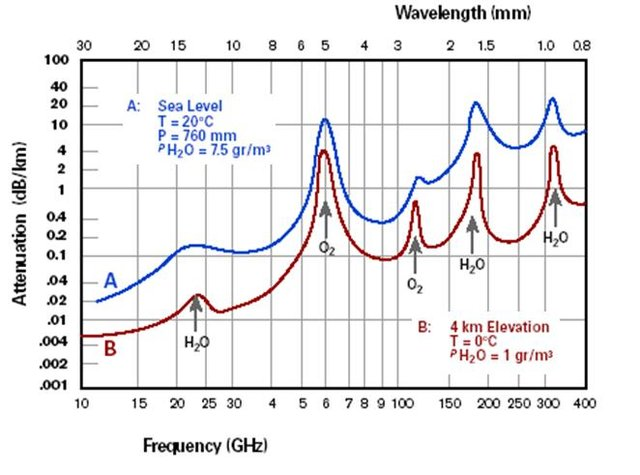
\includegraphics[width=0.8\textwidth]{res/atm-absorp.jpg}
    \caption{Atmospheric absorption in dB per kilometer, from \cite{e-band-ammar}}
    \label{fig:atmospheric-abs}
\end{figure}



\begin{table}[]
    \begin{tabular}{cllll}
    \hline
    {\ul \textbf{Case}} & \multicolumn{1}{c}{{\ul \textbf{Orbit}}} & \multicolumn{1}{c}{{\ul \textbf{Terminal}}} & \multicolumn{1}{c}{{\ul \textbf{Band}}} & \multicolumn{1}{c}{{\ul \textbf{Polarization Reuse}}} \\ \hline
    1                   & GEO                                      & VSAT                                        & Ka                                      & Disabled                                              \\ \hline
    2                   & GEO                                      & VSAT                                        & Ka                                      & Enabled                                               \\ \hline
    3                   & GEO                                      & VSAT                                        & Ka                                      & Enabled                                               \\ \hline
    4                   & GEO                                      & Handheld                                    & S                                       & Disabled                                              \\ \hline
    5                   & GEO                                      & No                                          & Yes                                     & Enabled                                               \\ \hline
    6                   & LEO-600                                  & Yes                                         & Yes                                     & Disabled                                              \\ \hline
    7                   & LEO-600                                  & VSAT                                        & Ka                                      & Enabled                                               \\ \hline
    8                   & LEO-600                                  & VSAT                                        & Ka                                      & Enabled                                               \\ \hline
    9                   & LEO-600                                  & Handheld                                    & S                                       & Disabled                                              \\ \hline
    10                  & LEO-600                                  & Handheld                                    & S                                       & Enabled                                               \\ \hline
    11                  & LEO-1200                                 & VSAT                                        & Ka                                      & Disabled                                              \\ \hline
    12                  & LEO-1200                                 & VSAT                                        & Ka                                      & Enabled                                               \\ \hline
    13                  & LEO-1200                                 & VSAT                                        & Ka                                      & Enabled                                               \\ \hline
    14                  & LEO-1200                                 & Handheld                                    & S                                       & Disabled                                              \\ \hline
    15                  & LEO-1200                                 & Handheld                                    & S                                       & Enabled                                               \\ \hline
    \end{tabular}
    \caption{3GPP scenarios for NTN \label{tab:scenarios}}
    \end{table}

\subsection{ns-3 implementation}
The SIGNET research group at the University of Padova recently implemented a non-terrestrial channel model\footnote{The code is available at the following repository: \href{https://gitlab.com/mattiasandri/ns-3-ntn/-/tree/ntn-dev?ref_type=heads}{gitlab.com/mattiasandri}} for the ns-3 network simulator based on the \ac{3GPP} specifications described in the standard \cite{3gpp-tr-38.811}.
This channel model enables full-stack end-to-end simulations considering different \ac{NTN} scenarios \cite{Sandri_2023}.

\section{Implemented scenario}

This section aims to describe the reference scenario that was implemented in the ns-3 simulator in order to test the feasibility of the implementation of 5G \ac{NR} protocol suite in a non-terrestrial communication setting. 